\section{cardinalità}
\label{sec:cardinali}

\begin{definition}[cardinalità]
  Diremo che due insiemi $A$ e $B$ hanno la stessa \emph{cardinalità}%
\mymargin{cardinalità}%
\index{cardinalità} 
  (oppure sono \emph{equipotenti}) 
  \index{equipotenza}%
  \index{insiemi!equipotenti}%
  \index{insieme!equipotente}%
  se esiste una funzione bigettiva $f\colon A \to B$.
  Scriveremo in tal caso:
  \[
    \# A = \# B.  
  \] 
  Se esiste una funzione iniettiva $f\colon A\to B$ significa che 
  $A$ ha la stessa cardinalità di un sottoinsieme di $B$ (in quanto $f\colon A \to f(A)$
  risulta essere bigettiva). Scriveremo in tal caso:
  \[
    \# A \le \#B.
  \]
\end{definition}

Intuitivamente se due insiemi hanno la stessa cardinalità 
significa che hanno lo stesso numero di elementi.
Ma la precedente definizione riesce a catturare tale concetto senza dover 
ricorrere al concetto di numero. 
Questo ha il vantaggio di rendere questa definizione applicabile 
a qualunque insieme, anche con \emph{infiniti} elementi.

Si osservi che non abbiamo dato una definizione di $\#A$ e quindi non stiamo 
definendo cos'è la cardinalità di un insieme ma stiamo soltanto definendo 
una relazione tra insiemi che 
denotiamo, impropriamente, utilizzando una uguaglianza: $\#A = \#B$.

E' ovvio che $\#A = \#A$ in quanto l'identità $\id_A$ è bigettiva.
E' anche chiaro che se $\#A = \#B$ e $\#B = \#C$ allora $\#A = \#C$ in quanto 
componendo tra loro due funzioni bigettive si ottiene ancora una funzione 
bigettiva. 
Infine se $\#A = \#B$ allora $\#A \le \#B$ (in quanto le funzioni bigettive 
sono iniettive) ed è chiaro che se $\#A \le \#B$ e $\#B \le \#C$ allora 
$\#A\le \#C$ (in quanto composizione di funzioni iniettive è iniettiva).

Possiamo definire il simbolo inverso $\#A \ge \#B$ 
come $\#B\le \#A$.
Ovviamente se $A\subset B$ si ha $\#A \le \#B$.
Se $B\neq \emptyset$ 
il seguente teorema ci dice che $\#A \ge \#B$ 
è equivalente a dire che 
esiste $f\colon A \to B$
surgettiva. 
%
\begin{theorem}\label{th:95444}
  Sia $B\neq \emptyset$.
  Esiste $f\colon A\to B$ surgettiva 
  se e solo se esiste $g\colon B\to A$ iniettiva.
\end{theorem}
% 
\begin{proof}
Da un lato se esiste $g\colon B\to A$ iniettiva, allora $g$ è una bigezione 
tra $B$ e $g(B)$. La funzione inversa $f\colon g(B) \to B$ 
\mynote{Questa funzione $f$ si chiama 
\emph{inversa sinistra}
\index{inversa!sinistra}%
di $g$ in quanto si ha $f(g(y))=y$ per ogni $y\in B$}
può essere estesa a tutto $A$ fissando un valore qualunque 
(questo si può fare se $B$ non è vuoto) nei punti di $A\setminus g(B)$
ottenendo quindi una funzione surgettiva da $A$ in $B$.
D'altro lato se esiste una funzione $f\colon A\to B$ surgettiva,
per ogni $b\in B$ l'insieme $f^{-1}(\ENCLOSE{b})$ non è mai 
vuoto e quindi è chiaro che debba esistere 
una funzione $g\colon B\to A$ tale che $g(b)$ è un qualunque elemento 
di tale insieme
\mynote{Questa funzione $g$ si chiama 
\emph{inversa destra} 
\index{inversa!destra}%
di $f$ 
in quanto $f(g(y))=y$ per ogni $y\in B$}
(qui si utilizza l'assioma~\ref{axiom:AC} discusso più sotto). 
Chiaramente $g$ è iniettiva.
\end{proof}

Nella dimostrazione del teorema precedente abbiamo utilizzato il seguente assioma 
della teoria degli insiemi che, sorprendentemente, non è conseguenza degli assiomi 
che abbiamo già introdotto finora.

\begin{axiom}[della scelta]%
  \label{axiom:AC}%
  \index{assioma!della scelta}%
  \index{scelta!assioma della}%
  \index{AC}%
  Sia $F\colon A \to \mathcal P(B)$
  una funzione tale che $F(a)\neq \emptyset$ 
  per ogni $a\in A$. Allora esiste una funzione
  $f\colon A \to B$ tale che $f(a)\in F(a)$
  per ogni $a\in A$.
\end{axiom}

L'assioma della scelta (denotato spesso con \emph{$AC$}%
\mymargin{$AC$}%
\index{AC}, \emph{axiom of choice})
è un assioma per certi versi controverso
e alcuni matematici preferiscono non utilizzarlo nelle loro dimostrazioni.
Il sistema formale che definisce la teoria degli insiemi senza 
introdurre l'assioma della scelta 
si chiama \emph{$ZF$}%
\mymargin{$ZF$}%
\index{ZF} (Zermelo-Fraenkel) mentre 
se si aggiunge l'assioma della scelta (choice) la teoria si chiama 
\emph{$ZFC$}%
\mymargin{$ZFC$}%
\index{ZFC}.

Grazie all'assioma della scelta è anche possibile dimostrare 
che dati due insiemi $A$ e $B$ le loro cardinalità
si possono confrontare: $\#A\le \#B$ oppure 
$\#B\le \#A$. 
La dimostrazione però diventa complicata e va oltre i nostri scopi.

\begin{theorem}
  \label{th:cardinale_totale}%
  Se $A$ e $B$ sono insiemi qualunque si ha $\#A\le \#B$ oppure $\#B\le \#A$.
\end{theorem}

Il seguente teorema dimostra invece la proprietà antisimmetrica 
della relazione tra cardinalità. 

\begin{theorem}[Cantor-Bernstein]%
  \label{th:cantor_bernstein}%
  \index{teorema!di Cantor-Bernstein}%
  \index{Cantor-Bernstein!teorema di}%
  Se $\#A \le \#B$ e $\#B \le \#A$ allora $\#A = \#B$.
\end{theorem}
%
\begin{figure}
  \centering
  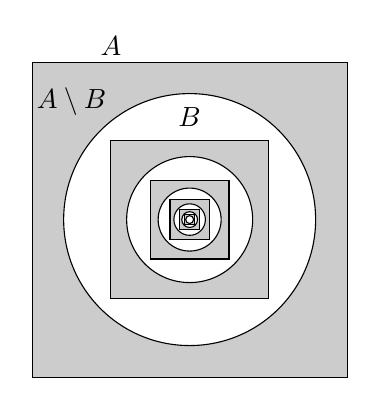
\begin{tikzpicture}
    \foreach \x in {1,0.5,0.25,0.25*0.5,0.25*0.25,0.25*0.25*0.5} {
      \path[draw,fill=black!20] (2*\x,2*\x)--(-2*\x,2*\x)--(-2*\x,-2*\x)--(2*\x,-2*\x)--cycle;
      \draw[fill=white] (0,0) circle (1.6*\x);
    };
    \node at (-1.0,2.2) {$A$};
    \node at (-1.5,1.5) {$A\setminus B$};
    \node at (0,1.3) {$B$};
%    \node at (-0.75,0.75) {$$};
  \end{tikzpicture}
  \caption{
  Nella dimostrazione del teorema di Cantor-Bernstein
  $A$ è rappresentato da un quadrato e $B$ da un cerchio contenuto
  in $A$. L'immagine di $A$ in $B$ è rappresentata da un quadrato contenuto
  in $B$ e così via. La parte ombreggiata è l'insieme $D$.
  }
  \label{fig:omotetia}
\end{figure}
%
\begin{proof}
Per ipotesi sappiamo che esiste
$g\colon B\to A$ iniettiva. 
Posto $B'=g(B)$ risulta che $g\colon B\to B'$ è bigettiva.
Ma allora dimostrare che esiste una bigezione tra $A$ e $B$ 
è equivalente a dimostrare che esiste una bigezione tra 
$A$ e $B'$. 
Dunque senza perdere di generalità, sostituendo $B'$ a $B$ 
possiamo supporre che sia $B\subset A$.

Essendo per ipotesi $\#A \le \#B$ esiste $f\colon A \to B$ iniettiva.
Intuitivamente l'idea è quella di definire l'insieme
\[
 D = (A\setminus B)  
 \cup f(A\setminus B) 
 \cup f(f(A\setminus B)) 
 \cup \dots
\]
e di definire la bigezione $\phi \colon A \to B$ 
utilizzando $f$ sull'insieme $D$ e lasciando fisso
il resto.

Per farlo in maniera rigorosa
consideriamo la famiglia di insiemi 
$\F = \{X \subset A \colon X \supset A \setminus B, f(X) \subset X\}$ 
e definiamo $D = \bigcap \F$.
Osserviamo che $A \in \F$ quindi $\F\neq \emptyset$.
Abbiamo in pratica definito $D$ come il più piccolo 
sottoinsieme di $A$ che viene mandato in se stesso da $f$.

E' facile verificare che $f(D) \subset D$ infatti dato $x\in D$ per ogni $X\in \F$ deve essere $x\in X$ ma allora $f(x) \in X$ (per come è definito $\F$), dunque $f(x) \in D$. 
In modo analogo si dimostra che $D\supset A\setminus B$ e dunque concludiamo che $D\in \F$.

Verifichiamo ora che $f(D)=D\cap B$. Da un lato se $x\in D$ allora
$f(x) \in f(D)\subset D$ e $f(x)\subset f(A)\subset B$ da cui $f(x) \in D\cap B$.
Dall'altro lato se $y\in D \cap B$ e non fosse $y \in f(D)$
allora potremmo considerare l'insieme $X=D\setminus\{y\}$
e osservare che $X\in \F$.
Infatti in primo luogo $X \supset A \setminus B$ in quanto $D$ ha questa proprietà e $y \in B$.
Inoltre dato qualunque $x \in X$ visto che $X\subset D$ allora
$f(x) \in f(D)$ e, per ipotesi,
$y\not \in f(D)$ dunque $f(x)\neq y$ da cui $f(x) \in X$.
Dunque $X\in \F$ ma allora dovrebbe essere $D\subset X$ mentre
per costruzione abbiamo $y\in D$ ma non in $X$.

% Avendo visto che $f(D)=D\cap B$ possiamo facilmente
% osservare che $f(A\setminus D) \subset A \setminus D$.
% Infatti $f(A\setminus D)\subset f(A)=B$ e quindi
% $f(A\setminus D)\cap D \subset D \cap B = f(D)$
% ma essendo $f$ iniettiva si deve avere
% $f(A\setminus D) \cap f(D)=\emptyset$.

Possiamo allora definire $\phi \colon A \to B$
\[
\phi(x) =
\begin{cases}
   f(x) & \text{se $x\in D$}, \\
   x & \text{altrimenti.}
\end{cases}
\]
Chiaramente $\phi$ è iniettiva in quanto $f$ è iniettiva e manda $D$ in $D$
e l'identità è iniettiva e manda $A\setminus D$ in $A\setminus D$.

Per dimostrare che $\phi$ è suriettiva consideriamo qualunque $y \in B$.
Se $y\not \in D$ allora $\phi(y)=y$.
Se invece $y\in D$ essendo $y\in D\cap B = f(D)$ esisterà $x\in D$ tale
che $\phi(x) = f(x) = y$.
\end{proof}

Ricordiamo il teorema~\ref{th:cardinali_finiti}
che ci dice che $A$ è un insieme finito se e solo se 
esiste $n\in\NN$ 
tale che $\#A = \#[n]$ dove abbiamo posto $[n]=\ENCLOSE{k\in \NN, k<n}
=\ENCLOSE{0,\dots,n-1}$.
Ora possiamo osservare che $\#A=n$ è una abbreviazione di $\#A = \#[n]$.

La cardinalità di $\NN$ viene a volte indicata con il simbolo
\index{$\aleph_0$}%
\index{aleph}%
$\aleph_0$ dunque potremo scrivere  
\[
    \# A = \aleph_0, \qquad
    \#A \le \aleph_0, \qquad
    \# A\ge \aleph_0
\]
per significare rispettivamente 
\[
  \# A = \# \NN, \qquad
  \# A \le \# \NN, \qquad
  \# A \ge \# \NN.  
\]
\mynote{%
Il simbolo $\aleph$ è la prima lettera dell'alfabeto ebraico 
e si legge \emph{aleph}. 
\\
Ricordiamo (teorema~\ref{th:unicitaN}) che gli insiemi 
$\NN$ che soddisfano gli assiomi di Peano sono tutti tra loro isomorfi 
e quindi, in particolare, hanno tutti la stessa cardinalità.
Abbiamo già osservato (teorema~\ref{th:esistenza_naturali}) 
che se $A$ è un insieme infinito esiste $N\subset A$
che soddisfa gli assiomi di Peano. 
L'inclusione $N\to A$ è iniettiva e quindi $\aleph_0 = \# \NN \le \# A$
per qualunque $A$ infinito.
In questo senso $\NN$ è il \emph{più piccolo} insieme 
infinito dunque $\aleph_0$ è la più piccola 
cardinalità infinita.
\\
Si potrebbe anche dimostrare che deve esistere una cardinalità $\aleph_1>\aleph_0$
che è la più piccola cardinalità maggiore di $\aleph_0$.
Sappiamo che $\# \mathcal P(\NN)>\# \NN$ ma curiosamente non è possibile dimostrare 
che $\aleph_1 = \# \mathcal P(\NN)$ (questa si chiama \emph{ipotesi del continuo}
\index{ipotesi!del continuo}%
\index{continuo!ipotesi del}%
in quanto vedremo nel teorema~\ref{th:cantor_secondo} che $\# \mathcal P(\NN)=\#\RR$
e l'insieme $\RR$ viene chiamato \emph{continuo} là dove $\NN$ 
viene chiamato \emph{discreto}).
Dunque l'ipotesi del continuo è un ulteriore assioma che potrebbe essere 
aggiunto agli assiomi della teoria degli insiemi: 
non esistono insiemi con cardinalità strettamente compresa tra 
le cardinalità di $\NN$ e di $\mathcal P(\NN)$.
}%

Abbiamo già osservato che $\NN$ è un insieme infinito e dunque 
anche $\ZZ$, $\QQ$ e $\RR$ sono infiniti.
Per gli insiemi finiti se $A\subset B$ ma $A\neq B$ risulta $\#A < \# B$
in quanto $\#A - \#B = \#(B\setminus A) > 0$. 
Dobbiamo però osservare che lo stesso non vale per gli insiemi infiniti.
In effetti la funzione $s\colon \NN \to \NN$ definita da $s(x)=x+1$
risulta essere una bigezione tra $\NN$ e $\NN\setminus\ENCLOSE{0}$. 
Dunque $\#\NN = \#(\NN\setminus\ENCLOSE{0})$ 
nonostante la differenza tra i due insiemi $\ENCLOSE{0}$ abbia 
cardinalità $1$. 
Anche l'insieme dei numeri pari o l'insieme 
dei quadrati perfetti (come aveva notato già Galileo)
hanno la stessa cardinalità di $\NN$ in quanto le funzioni $n\mapsto 2n$
e la funzione $n\mapsto n^2$ sono iniettive.

Non è difficile trovare una funzione iniettiva da $\ZZ$ in $\NN$
(lo lasciamo per esercizio): questo dimostra che anche $\#\ZZ = \# \NN$.

Cantor dimostra addirittura che $\#\QQ = \#\NN$: 
per farlo utilizza il seguente.

\begin{theorem}[primo metodo diagonale di Cantor]
\label{th:Cantor_primo}%
\index{Cantor!primo metodo diagonale}%
L'insieme $\NN \times \NN$ ha la stessa cardinalità di $\NN$. Di conseguenza
\[
  \# \NN = \# \ZZ = \# \QQ.
  \]
\end{theorem}
%
\begin{proof}[Idea di dimostrazione]
  Numerare le caselle di una scacchiera infinita
  come in Figura~\ref{fig:cantor1}.
  
  Visto che è piuttosto facile trovare una funzione iniettiva 
  da $\QQ$ in $\NN \times \ZZ$ si deduce facilmente che $\#\QQ = \#\NN$.
\end{proof}

\begin{figure}
  \begin{tabular}{c|ccccccc}
   $m$ & $\ddots$ & $\ddots$ & $\ddots$ & $\ddots$ & $\ddots$ & $\ddots$\\
   $\vdots$ & $\ddots$ & $\ddots$ & $\ddots$ & $\ddots$ & $\ddots$ & $\ddots$\\
   3 & 9 & $\nwarrow$ & $\ddots$  & $\ddots$ & $\ddots$ & $\ddots$\\
   2 & 5 & 8 & 12 & $\ddots$  & $\ddots$ & $\ddots$\\
   1 & 2 & 4 & 7 & 11 & $\ddots$  & $\ddots$\\
   0 & 0 & 1 & 3 & 6 & 10 & $\ddots$ \\ \hline
     & 0 & 1 & 2 & 3 & 4 & $\dots$ & $n$
  \end{tabular}
  \caption{
    La numerazione diagonale delle caselle
    di una scacchiera infinita. Si potrebbe verificare
    che il numero presente nella casella di coordinate $(n,m)$
    si scrive come $f(n,m) = \frac{(n+m+1)(n+m)}{2}+m$
    ed è una funzione bigettiva $f\colon \NN\times\NN \to\NN$.}
  \label{fig:cantor1}
\end{figure}

A questo punto si potrebbe pensare che
tutti gli insiemi infiniti siano numerabili.
Invece preso un qualunque insieme (anche infinito)
esiste sempre un insieme con cardinalità maggiore,
come dimostrato nel seguente teorema che è un piccolo gioiello della logica.
In effetti il metodo utilizzato è assimilabile al paradosso del mentitore 
ed è la stessa idea usata nel paradosso di Russell (teorema~\ref{th:Russell}).
\mynote{L'insieme $\mathcal P(A)$ è l'insieme delle parti, 
definito a pag.~\pageref{def:insieme_parti}}%
%
\begin{theorem}[Cantor]%
\index{Cantor!cardinalità dell'insieme delle parti}%
\index{Teorema di!Cantor}%
\label{th:Cantor}%
  Se $A$ è un qualunque insieme allora $\# \mathcal P(A) > \# A$.
\end{theorem}
%
\begin{proof}
  E' chiaro che $\# A \le \#\mathcal P(A)$ in quanto 
  la funzione $f\colon A \to \mathcal P(A)$ definita da $f(x)=\ENCLOSE{x}$
  è ovviamente iniettiva.

  Supponiamo allora per assurdo che esista $f\colon A\to \mathcal P(A)$
  bigettiva e consideriamo l'insieme 
  \[
    C = \ENCLOSE{x\in A \colon x\not\in f(x)}.  
  \]
  Se $f$ fosse surgettiva dovrebbe esistere $c\in A$ tale che $f(c) = C$.
  Possiamo allora chiederci se $c\in C$ e scoprire che, 
  per definizione di $C$ la proposizione $c\in C$ è equivalente 
  a $c\not\in f(c) = C$. 
  Dunque $c\in C \iff c\not\in C$, che è assurdo.
\end{proof}
%
\begin{corollary}[non esiste l'insieme di tutti gli insiemi]
  Se esistesse un insieme $\mathcal U$ (universo) 
  tale che $\forall x\colon x \in U$, allora 
  si avrebbe $\mathcal \P(\mathcal U) \subset \mathcal U$
  contraddicendo il teorema precedente.
\end{corollary}
%
Per quanto riguarda l'insieme $\RR$ si
scopre in effetti che $\#\RR > \#\NN$
(sempre grazie a Cantor, teorema~\ref{th:cantor_secondo} qui sotto)
e si potrebbe dimostrare che effettivamente $\#\RR = \#\mathcal P(\NN)$.

\begin{theorem}[secondo metodo diagonale di Cantor]
  \label{th:cantor_secondo}
L'insieme di Cantor
\[
  C = \{r(\vec a)\colon \vec a \in \ENCLOSE{0,2}^\NN\}
\]
ha cardinalità
\[
\# C = \# \mathcal P(\NN).
\]
In particolare $\#\RR > \#\NN$.
\end{theorem}
%
\begin{proof}
Consideriamo la funzione $r$ definita nel capitolo~\ref{sec:decimali} che associa 
ad una sequenza di cifre binarie il corrispondente numero reale.
Vogliamo verificare che $r\colon \ENCLOSE{0,2}^\NN \to \closeinterval{0}{1}$
è iniettiva.
Abbiamo già visto in generale che $r(\vec a) = r(\vec b)$ solamente 
se la prima cifra diversa in $\vec a$ e $\vec b$ differisce di una unità.
Ma siccome tutte le cifre di $\vec a$ e $\vec b$ per ipotesi sono $0$ oppure 
$2$, non differiscono di una unità e quindi $r$ è iniettiva.
Dunque $\# C = \#\ENCLOSE{0,2}^\NN$.
D'altra parte $\#\ENCLOSE{0,2}^\NN = \#\mathcal P(\NN)$ in quanto 
ogni $\vec a \in \ENCLOSE{0,2}^\NN$ può essere messo in corrispondenza 
biunivoca con l'insieme $\vec a^{-1}(\ENCLOSE{0})$ degli indici $k\in \NN$
per cui $a_k=0$.

Dal teorema~\ref{th:Cantor} deduciamo che $\# C = \#\mathcal P(\NN) > \#\NN$ 
e visto che $C\subset \RR$ a maggior ragione $\# \RR \ge \# C >\#\NN$.

D'altra parte possiamo mostrare che $\#\RR \le \# \mathcal P(\NN)$
in quanto possiamo costruire una funzione $f\colon \RR \to \mathcal P(\QQ)$
in questo modo:
\[
f(x) = \ENCLOSE{q\in \QQ\colon q<x}.
\]
Per la densità di $\QQ$ in $\RR$ sappiamo che se $x<y$ 
esiste $q\in \QQ$ con $x<q<y$ e dunque $q\in f(y)\setminus f(x)$ 
da cui $f(x)\neq f(y)$. 
Dunque $f$ è iniettiva, che significa $\#\RR\le \# \mathcal P(\QQ)$
Ma $\#\NN = \#\QQ$ dunque $\#\mathcal P(\QQ) = \#\mathcal P(\NN)$ 
e la dimostrazione è conclusa.
\end{proof}

L'insieme $C$ definito nella precedente dimostrazione con $d=3$ 
è lo stesso \emph{insieme di Cantor}%
\mymargin{insieme di Cantor}%
\index{insieme!di Cantor}
\index{Cantor!insieme di}% 
considerato nell'esempio~\ref{ex:insieme_Cantor}.
Infatti si potrebbe mostrare facilmente che 
$C=\frac 1 3 C \cup (\frac 2 3 + \frac 1 3 C)$.

